\documentclass[conference]{IEEEtran}
\usepackage{graphicx}
\usepackage{booktabs}
\usepackage{textcomp}
\usepackage{url}
\graphicspath{{../../../figures/v2/}}
\newcommand{\cdiff}{\textit{C.~difficile}}

\begin{document}

\title{Healthy reference ranges for gut metagenomes,\\shipped with the pipelines that measure them}
\author{\IEEEauthorblockN{[Authors]}\IEEEauthorblockA{[Affiliation]}}
\maketitle

\begin{abstract}
A gut metagenome profile lists hundreds of abundances but does not say which are unusual. Clinical laboratories answer that question with reference intervals measured in healthy people on the same assay; metagenomics has no equivalent, so every study judges its cases against its own controls and a single sample cannot be read at all. We present refmb, which ships two standard analysis pipelines together with baselines of healthy adults processed exactly the same way, and reports every taxon, gene family and pathway of a new sample as a percentile among those adults. The assembly pipeline reproduces MGnify v5 (1{,}941 adults, 26 studies); the read pipeline reproduces curatedMetagenomicData~3 (6{,}494 adults, 19 studies). Healthy cohorts the baselines never saw fall outside the healthy range at close to the expected 5\%. In studies left out of training, percentiles separate cases from controls better than raw abundances, and a sparse score built on them matches the published Gut Microbiome Wellness Index~2 (mean AUROC 0.75 vs.\ 0.72) without its training overlap. Unlike a score, percentiles explain themselves: they show the loss of obligate anaerobes in individual \cdiff{} patients, the depletion of butyrate producers across nine colorectal cancer cohorts, and the genera that place Hadza hunter-gatherers outside an industrialized healthy range.
\end{abstract}

\begin{IEEEkeywords}
gut microbiome, metagenomics, reference ranges, interpretability, reproducible pipelines
\end{IEEEkeywords}

\section{Introduction}

A blood test is read against a reference interval: the spread of values seen in healthy people measured on the same assay~\cite{horn2003}. Gut metagenomics has no such interval. Profilers turn a stool sample into the abundances of hundreds of taxa, genes and pathways~\cite{beghini2021,richardson2023}, but whether any one of them is unusual is decided study by study, against that study's own controls. So a single sample cannot be interpreted on its own; effect sizes from different studies are not on a common scale, a known obstacle to meta-analysis~\cite{duvallet2017}; and the usual alternative, a health index condensing a profile into one number~\cite{gupta2020,chang2024}, reports that a sample looks diseased without saying which features are unusual or by how much.

The gap is not for want of healthy data; tens of thousands of healthy gut metagenomes are public. But a range is only valid for data processed the same way, since profiles from different pipelines are not interchangeable~\cite{sczyrba2017}, so a range and the software that produced it must travel together --- and public cohorts are shipped as per-sample tables that must still be re-processed before anything new can be compared with them.

refmb closes the gap by shipping the pipeline and the baseline as one object (Fig.~\ref{fig:overview}). Two pipelines reproduce two public resources, an assembly-based one (MGnify v5~\cite{richardson2023}) and a read-based one (curatedMetagenomicData~3, cMD3~\cite{pasolli2017}), and each carries a baseline of healthy adults from that resource, stored as summary statistics only: no samples, a few megabytes. A user runs a pipeline on raw reads and receives, for every feature, its percentile among healthy adults, a call (within, below or above the 2.5th--97.5th percentile range), and the features most healthy adults carry but this sample lacks. We show that this scale carries as much disease information as a published health index, and that unlike a single score it says what is unusual --- in one patient, across cohorts of one disease, and in a healthy population an industrialized baseline does not fit.

\begin{figure*}[t]
\centering
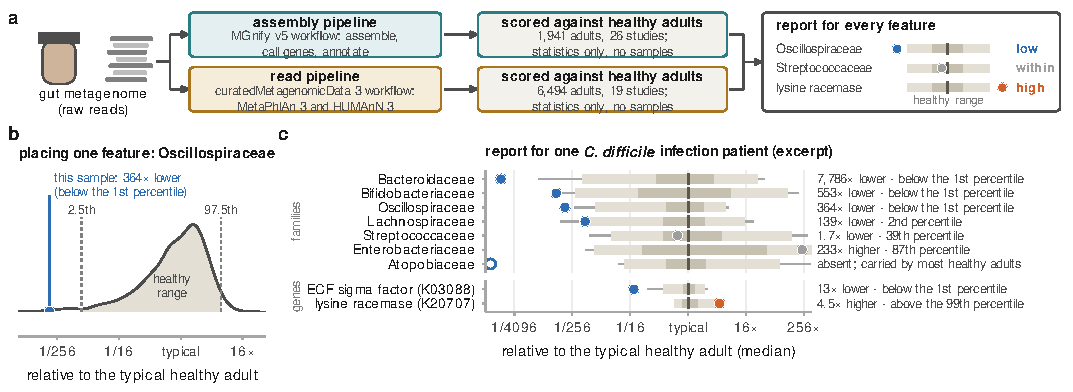
\includegraphics[width=\textwidth]{fig1.pdf}
\caption{\textbf{refmb places a new sample among healthy adults measured the same way.} (a) Raw reads go through either pipeline and are scored against the baseline bundled with it; the report gives a percentile and a call for every feature. (b) How one feature is placed: the distribution of \textit{Oscillospiraceae} in 1{,}922 healthy adults, its 2.5th--97.5th percentile healthy range, and one \cdiff{} infection patient, 364$\times$ below the typical healthy adult. (c) Part of that patient's report. Grey bar, healthy range; darker bar, middle half of healthy adults; tick, typical healthy adult; whisker, 1st--99th percentile; dot, this sample; open ring, expected but absent. \textit{Enterobacteriaceae} is 233$\times$ above typical and still inside the (wide) healthy range.}
\label{fig:overview}
\end{figure*}

\section{Methods}

\subsection{Cohorts and pipelines}

\emph{Assembly pipeline.} We inventoried 19{,}437 MGnify v5 analyses from 130 studies and kept 9{,}195 gut metagenomes (one per sample, 69 studies), of which 8{,}742 passed assembly quality filters ($\geq$5~Mb assembled, $\geq$20 of 52 single-copy marker genes; Fig.~\ref{fig:methods}b); health status, age and sex come from a manual curation of the study and sample metadata. A pinned container reproduces the MGnify v5 workflow from raw reads: metaSPAdes 3.15.3~\cite{nurk2017} or MEGAHIT 1.2.9~\cite{li2015}, Prodigal 2.6.3~\cite{hyatt2010} and FragGeneScan gene calls, DIAMOND~\cite{buchfink2015} against UniRef90 for taxonomy, and eggNOG-mapper~\cite{huerta2017}, KOfam~\cite{aramaki2020} and InterProScan for function. Taxa are coverage-weighted proportions of assigned sequence; genes are copies per genome, scaled by marker-gene coverage~\cite{nayfach2015}.

\emph{Read pipeline.} We took the 9{,}246 cMD3 MetaPhlAn~3 profiles of 37 studies with their curated metadata~\cite{antonello2025} and kept 7{,}478 adult stool controls whose profile is at least 90\% resolvable to an NCBI family. The pipeline is MetaPhlAn 3.0.14~\cite{beghini2021} with the mpa\_v30 markers on untrimmed reads, as cMD3 did, with optional HUMAnN~3 tables grouped into KEGG orthologs (KOs) and MetaCyc pathways~\cite{caspi2020}.

\subsection{Baselines}

Both baselines are built by the same rules. Compositional layers are transformed to centred log-ratios~\cite{aitchison1982} over features present in at least 5\% of baseline samples, and for each feature the baseline stores its prevalence per sequencing-depth class and its 1st--99th percentiles among the samples that carry it, with equal weight per study so that large studies do not dominate. A new sample is normalized by the stored rules and its percentile interpolated between the stored quantiles. A feature is \textbf{low} or \textbf{high} outside the 2.5th--97.5th percentile range, and \textbf{expected but missing} when at least 70\% of healthy samples of its depth class carry it and this one does not. The \emph{fraction outside} is the share of a sample's features outside the range; for a healthy sample it should be about 5\%.

\begin{table}[t]
\caption{The two baseline cohorts}
\label{tab:cohorts}
\centering
\scriptsize
\setlength{\tabcolsep}{4pt}
\begin{tabular}{lrr}
\toprule
 & Assembly (MGnify v5) & Read (cMD3) \\
\midrule
Screened, samples (studies) & 19{,}437 (130) & 9{,}246 (37) \\
Baseline healthy adults & 1{,}941 (26) & 6{,}494 (19) \\
Countries & 24 & 16 \\
Median age, y (\% recorded) & 53 (52\%) & 44 (85\%) \\
Women (\% recorded) & 52\% (66\%) & 59\% (91\%) \\
Taxonomic features scored & 2{,}271 & 422 \\
Functional features scored & 13{,}401 & 4{,}941 \\
Held-out healthy adults & 233 (3) & 317 (3) \\
Case/control samples & 2{,}294 (11) & 1{,}437 (15) \\
\bottomrule
\end{tabular}
\end{table}

\begin{figure*}[t]
\centering
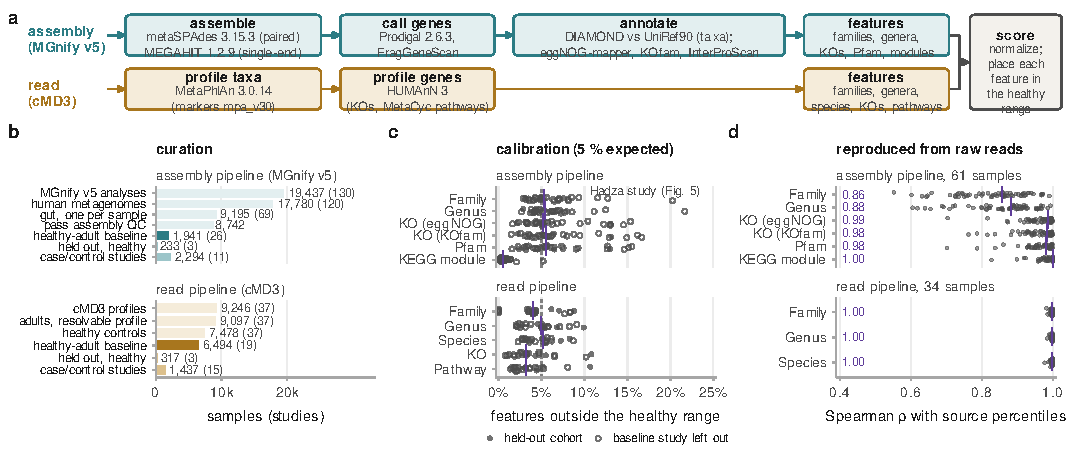
\includegraphics[width=\textwidth]{fig2.pdf}
\caption{\textbf{Each pipeline is paired with a baseline curated from a public resource by fixed rules.} (a) The two workflows and the shared scoring step. (b) From public resource to baseline, with the evaluation sets set aside first; counts are samples (studies). (c) Share of features outside the healthy range for healthy cohorts the baseline never saw and for each baseline study scored against a baseline rebuilt without it; violet tick, median per layer. The one clear outlier is the Hadza study of Fig.~\ref{fig:population}. (d) Both pipelines reproduce the percentiles of the source resource when re-run from deposited raw reads.}
\label{fig:methods}
\end{figure*}

\subsection{Evaluation}

No sample was ever compared with a baseline that contained it: baseline studies were scored against a baseline rebuilt without them, cases and controls of a disease study always against the same baseline, and 30 samples deposited in two cMD3 studies against a baseline without their duplicate, never split across a training/test boundary.

For a case/control study with at least 15 cases and 15 controls, a feature's \emph{shift} is the median percentile of cases minus that of the same study's controls; it is significant at $\geq$10 points with $q \leq 0.05$ (Mann--Whitney, Benjamini--Hochberg~\cite{benjamini1995} within study and layer), and \emph{consistent} when it holds in the same direction in at least two studies of one condition.

For the benchmark, a random forest~\cite{breiman2001} trained on all other case/control studies classified each left-out study from percentiles, raw abundances or alpha diversity; on the read pipeline we also scored the Gut Microbiome Health Index (GMHI)~\cite{gupta2020} and the Gut Microbiome Wellness Index~2 (GMWI2)~\cite{chang2024} as published, without retraining. To compete with them on their own ground we pre-specified a sparse health score on refmb output: an L1-penalized logistic regression on the percentiles, the fraction outside, the number of missing features and species presence (which captures disease-associated taxa too rare in healthy adults for a percentile). Model and features were fixed before results were seen, each study was scored by a model trained without it, and the penalty was chosen inside the training studies only.

\section{Results}

\subsection{The baselines are calibrated and the pipelines reproduce their sources}

Healthy adults a baseline never saw should fall outside its healthy range about 5\% of the time, and they do: the median over held-out cohorts and left-out baseline studies is 5.3\% of families in the assembly baseline and 4.0\% in the read baseline, with the same picture for gene families and pathways (Fig.~\ref{fig:methods}c). Re-run from deposited raw reads, both pipelines return the percentiles of the resource they reproduce: median Spearman $\rho$ 0.99 for gene families and 0.86 for families in 61 MGnify samples, 1.00 across layers in 34 cMD3 samples (Fig.~\ref{fig:methods}d). The ranges are usable by anyone running the pipeline, not only by us.

\subsection{Percentiles carry as much disease information as a published index}

\begin{figure}[t]
\centering
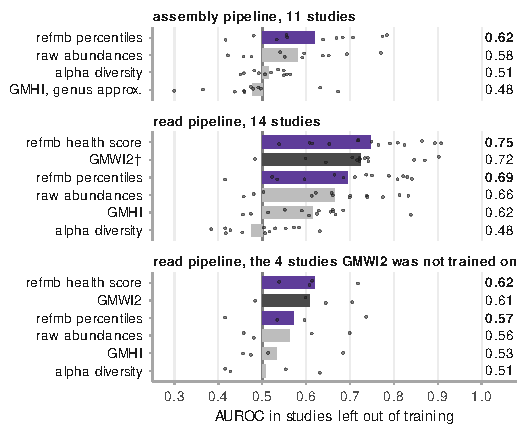
\includegraphics[width=\columnwidth]{fig3.pdf}
\caption{\textbf{In studies left out of training, refmb output separates cases from controls at least as well as published health indices.} Bars are means over studies, dots are individual studies; 0.5 is chance. $\dagger$GMWI2's training set includes samples from 10 of these 14 studies, so the bottom panel, the four studies it never saw, is its fair comparison.}
\label{fig:benchmark}
\end{figure}

Percentiles are a transformation of the profile, so the first question is whether they cost predictive power. They do not (Fig.~\ref{fig:benchmark}). On the assembly pipeline, across 11 studies each left out in turn, percentiles reach a mean AUROC of 0.62 against 0.58 for raw abundances (higher in 9 of 11 studies, $p = 0.021$), 0.51 for alpha diversity and 0.48 for a genus-level GMHI approximation; on the read pipeline, over 14 studies, 0.69 against 0.66 for raw abundances (10 of 14, $p = 0.039$) and 0.62 for the published GMHI (11 of 14, $p = 0.008$).

GMWI2, a supervised classifier, reaches 0.72, but its advantage is smaller than it appears: matching sequencing-run accessions and ENA projects shows its training set includes samples from 10 of these 14 studies. Our health score, which scored every study with a model trained without it, reaches 0.75 (higher in 10 of 14, $p = 0.22$); on the four studies neither model has seen the two are level (0.62 vs.\ 0.61) --- too few to separate them, but enough to say that a score built on reference ranges is competitive with the state of the art while remaining auditable.

Two cautions. Species presence inherits processing artifacts: \textit{[Collinsella] massiliensis} is present in most controls and absent from all cases of three cMD3 studies, a batch difference the model picks up as its strongest feature; a percentile-only variant is immune to it and does at least as well on the unseen studies (0.64). And trained only on studies containing both cases and controls, so that study identity cannot stand in for the label, the score still reaches 0.72.

\subsection{The same output explains itself, one patient at a time}

\begin{figure*}[t]
\centering
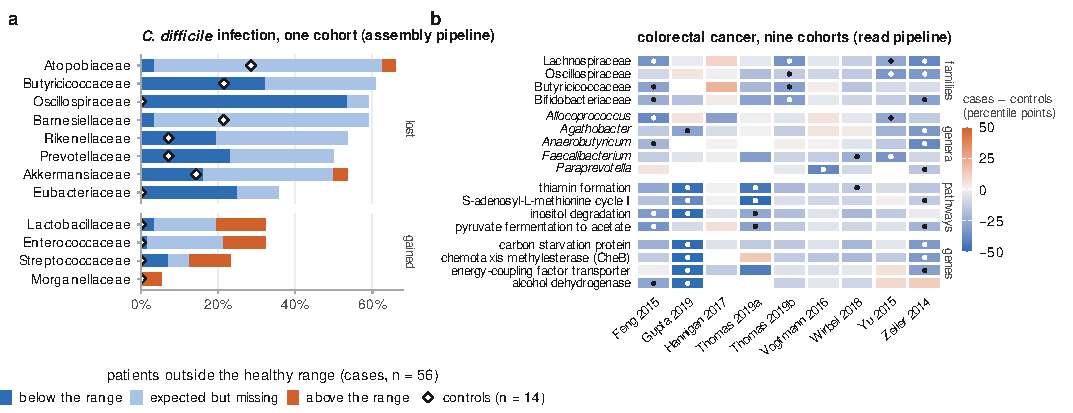
\includegraphics[width=\textwidth]{fig4.pdf}
\caption{\textbf{Reference ranges reproduce known disease associations, in one cohort and across nine.} (a) \cdiff{} infection: for the twelve families that separate cases from controls most, the share of the 56 patients in whom each is below the healthy range, expected but missing, or above it; diamonds mark the same share among the study's 14 controls. (b) Colorectal cancer: shift in median percentile between cases and the controls of the same cohort, for the taxa that shift consistently; dots mark significant shifts. A shift of $-30$ points means the same thing in every column, which is what makes the rows comparable.}
\label{fig:known}
\end{figure*}

A score says a sample looks diseased; a reference range says what is unusual in it, which is what the reader of a single report needs. In the \cdiff{} infection cohort of the assembly pipeline (56 patients, 14 controls, scored against a baseline rebuilt without the study), the obligate anaerobes drop out one family at a time: \textit{Oscillospiraceae} is below the healthy range in 54\% of patients and in no control, \textit{Atopobiaceae} and \textit{Barnesiellaceae} are expected but missing in 59\% and 55\%, and six further anaerobe families follow (Fig.~\ref{fig:known}a), while \textit{Lactobacillaceae}, \textit{Enterococcaceae} and \textit{Streptococcaceae} rise above the range in about one patient in eight and in no control --- the loss of anaerobic colonization resistance that defines the infection, recovered without using the controls.

The same report is available for a patient with no control group at all (Fig.~\ref{fig:overview}c): 17 of 103 assessed families below the range and none above, seven expected families missing, \textit{Bacteroidaceae} 7{,}786$\times$ below typical. \textit{Enterobacteriaceae} is 233$\times$ above typical and still inside the healthy range, at the 87th percentile --- a distinction no fold-change against a cohort mean can draw.

Across cohorts the shifts replicate. The nine colorectal cancer cohorts of the read pipeline show the depletion of butyrate-associated taxa that meta-analyses of the same studies report~\cite{thomas2019,wirbel2019}: \textit{Lachnospiraceae} is lower in cases in four cohorts (median $-35$ points), \textit{Oscillospiraceae} ($-33$), \textit{Bifidobacteriaceae} ($-29$), \textit{Lachnospira} and \textit{Fusicatenibacter} ($-25$) in three, and eight further genera in two (Fig.~\ref{fig:known}b). Because the unit is a percentile of one healthy baseline, these numbers read across columns, and the function layers extend the comparison beyond taxonomy: 100 pathways and 80 KOs shift consistently, 85 and 70 downward.

\subsection{A healthy population the baseline does not fit}

\begin{figure*}[t]
\centering
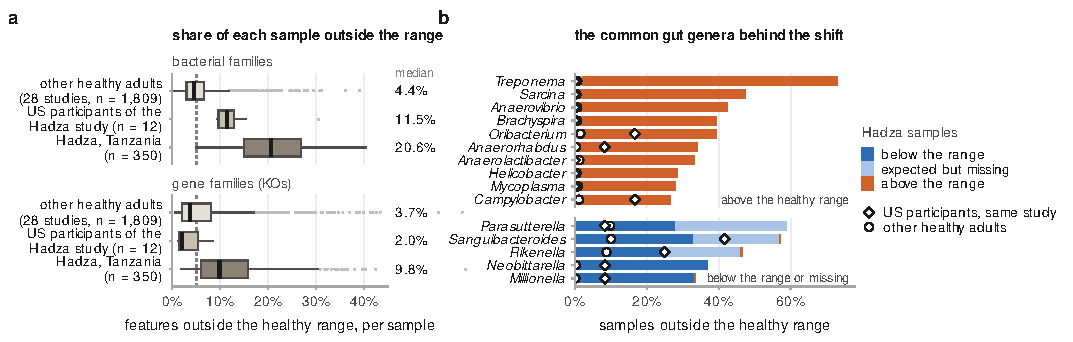
\includegraphics[width=\textwidth]{fig5.pdf}
\caption{\textbf{Hadza hunter-gatherers sit outside an industrialized healthy range, and the reference ranges name the genera responsible.} All samples are healthy adults scored out-of-sample. (a) Share of features outside the healthy range per sample. (b) The common gut genera that drive it, with the same study's US participants and the rest of the baseline for comparison.}
\label{fig:population}
\end{figure*}

A reference range is a claim about a population, and the honest test of one is a healthy population it was not built from. The baselines are dominated by European, North American and East Asian cohorts, and one baseline study stands out in the calibration (Fig.~\ref{fig:methods}c): the Hadza hunter-gatherers of Tanzania, sequenced alongside Nepali and Californian comparison groups~\cite{carter2023}. Scored out-of-sample, Hadza samples have a median 20.6\% of families outside the healthy range against 4.4\% for other healthy adults --- while the 12 US participants of the same study, processed identically, sit at 11.5\% (Fig.~\ref{fig:population}a). The excess is a property of the population, not of the sequencing.

The ranges also name the genera responsible, which a single score could not (Fig.~\ref{fig:population}b): \textit{Treponema} is above the healthy range in 71\% of Hadza samples, \textit{Sarcina} in 47\%, \textit{Anaerovibrio} in 42\% and \textit{Brachyspira} in 39\%, while \textit{Parasutterella}, \textit{Rikenella} and \textit{Sanguibacteroides} are low or missing in a quarter to a third --- the spirochaete- and fibre-fermenter-rich, industrialization-depleted taxa the Hadza microbiome is known for~\cite{carter2023}, recovered as deviations from an industrialized range rather than from a matched control group. The figure is a caution and a method at once: outside the populations a baseline was built from, the fraction outside is not a measure of ill health, and the per-feature output is what tells the two apart.

\section{Discussion}

refmb gives a single gut metagenome a position among healthy adults processed the same way, and ships that position with the software that produces it. As a predictor, a score built on it matches a published health index without that index's training overlap; as a report, it says which taxa, genes and pathways are unusual and by how much. One sample can be read without a control group, and because every sample lands on one scale, known associations replicate across cohorts --- and shipping the baseline as statistics only makes this reusable by anyone with reads.

The limits are visible in the same figures. The score is on par with GMWI2, not better, on the four studies neither model saw. Recovery of known biology is partial: two inflammatory bowel disease studies of the assembly pipeline show \textit{Blautia} and \textit{Faecalibacterium} higher in cases, against their well-replicated depletion~\cite{lloydprice2019,franzosa2019}, and taxa enriched in colorectal cancer but rare in healthy adults (\textit{Fusobacterium nucleatum}, \textit{Parvimonas}) fall below the prevalence filter and receive no percentile --- a reference range can only speak about features healthy people carry. The Hadza result bounds the claim geographically, population cannot be separated from study in either cohort, and a MetaPhlAn~4 baseline~\cite{blanco2023} would need a rebuild, which the tooling supports.

Reference intervals became useful in clinical chemistry once they were defined per assay, published with the method and re-derived for the populations being tested. refmb is an attempt to meet those three requirements for gut metagenomes. It is a Python package under the MIT license; the repository holds the code, container recipes for both pipelines and the documentation, and the baselines (assembly v0.8, read v0.2) and container image are deposited on Zenodo [DOI to be added].

{\footnotesize
\begin{thebibliography}{00}
\setlength{\itemsep}{0.3pt}
\bibitem{horn2003} P. S. Horn and A. J. Pesce, ``Reference intervals: an update,'' \emph{Clin. Chim. Acta}, vol. 334, no. 1--2, pp. 5--23, 2003.
\bibitem{beghini2021} F. Beghini \emph{et al.}, ``Integrating taxonomic, functional and strain-level profiling with bioBakery 3,'' \emph{eLife}, vol. 10, e65088, 2021.
\bibitem{richardson2023} L. Richardson \emph{et al.}, ``MGnify: the microbiome sequence data analysis resource in 2023,'' \emph{Nucleic Acids Res.}, vol. 51, no. D1, pp. D753--D759, 2023.
\bibitem{duvallet2017} C. Duvallet \emph{et al.}, ``Meta-analysis of gut microbiome studies identifies disease-specific and shared responses,'' \emph{Nat. Commun.}, vol. 8, 1784, 2017.
\bibitem{gupta2020} V. K. Gupta \emph{et al.}, ``A predictive index for health status from gut microbiome profiles,'' \emph{Nat. Commun.}, vol. 11, 4635, 2020.
\bibitem{chang2024} D. Chang \emph{et al.}, ``Gut Microbiome Wellness Index 2 enhances health status prediction,'' \emph{Nat. Commun.}, vol. 15, 7447, 2024.
\bibitem{sczyrba2017} A. Sczyrba \emph{et al.}, ``Critical Assessment of Metagenome Interpretation,'' \emph{Nat. Methods}, vol. 14, no. 11, pp. 1063--1071, 2017.
\bibitem{pasolli2017} E. Pasolli \emph{et al.}, ``Accessible, curated metagenomic data through ExperimentHub,'' \emph{Nat. Methods}, vol. 14, no. 11, pp. 1023--1024, 2017.
\bibitem{nurk2017} S. Nurk \emph{et al.}, ``metaSPAdes: a new versatile metagenomic assembler,'' \emph{Genome Res.}, vol. 27, no. 5, pp. 824--834, 2017.
\bibitem{li2015} D. Li \emph{et al.}, ``MEGAHIT: an ultra-fast single-node metagenomics assembler,'' \emph{Bioinformatics}, vol. 31, no. 10, pp. 1674--1676, 2015.
\bibitem{hyatt2010} D. Hyatt \emph{et al.}, ``Prodigal: prokaryotic gene recognition,'' \emph{BMC Bioinformatics}, vol. 11, 119, 2010.
\bibitem{buchfink2015} B. Buchfink, C. Xie, and D. H. Huson, ``Fast and sensitive protein alignment using DIAMOND,'' \emph{Nat. Methods}, vol. 12, no. 1, pp. 59--60, 2015.
\bibitem{huerta2017} J. Huerta-Cepas \emph{et al.}, ``Fast functional annotation by eggNOG-mapper,'' \emph{Mol. Biol. Evol.}, vol. 34, no. 8, pp. 2115--2122, 2017.
\bibitem{aramaki2020} T. Aramaki \emph{et al.}, ``KofamKOALA: KEGG Ortholog assignment,'' \emph{Bioinformatics}, vol. 36, no. 7, pp. 2251--2252, 2020.
\bibitem{nayfach2015} S. Nayfach and K. S. Pollard, ``Average genome size estimation improves comparative metagenomics,'' \emph{Genome Biol.}, vol. 16, 51, 2015.
\bibitem{antonello2025} G. Antonello and P. Manghi, ``Meta-analysis of 22,710 human metagenomes,'' Zenodo dataset v3, 2025, doi:10.5281/zenodo.17567900.
\bibitem{caspi2020} R. Caspi \emph{et al.}, ``The MetaCyc database---a 2019 update,'' \emph{Nucleic Acids Res.}, vol. 48, no. D1, pp. D445--D453, 2020.
\bibitem{aitchison1982} J. Aitchison, ``The statistical analysis of compositional data,'' \emph{J. R. Stat. Soc. B}, vol. 44, no. 2, pp. 139--160, 1982.
\bibitem{benjamini1995} Y. Benjamini and Y. Hochberg, ``Controlling the false discovery rate,'' \emph{J. R. Stat. Soc. B}, vol. 57, no. 1, pp. 289--300, 1995.
\bibitem{breiman2001} L. Breiman, ``Random forests,'' \emph{Mach. Learn.}, vol. 45, no. 1, pp. 5--32, 2001.
\bibitem{thomas2019} A. M. Thomas \emph{et al.}, ``Metagenomic analysis of colorectal cancer datasets,'' \emph{Nat. Med.}, vol. 25, no. 4, pp. 667--678, 2019.
\bibitem{wirbel2019} J. Wirbel \emph{et al.}, ``Global microbial signatures specific for colorectal cancer,'' \emph{Nat. Med.}, vol. 25, no. 4, pp. 679--689, 2019.
\bibitem{carter2023} M. M. Carter \emph{et al.}, ``Ultra-deep sequencing of Hadza hunter-gatherers recovers vanishing gut microbes,'' \emph{Cell}, vol. 186, no. 14, pp. 3111--3124, 2023.
\bibitem{lloydprice2019} J. Lloyd-Price \emph{et al.}, ``Multi-omics of the gut microbial ecosystem in IBD,'' \emph{Nature}, vol. 569, no. 7758, pp. 655--662, 2019.
\bibitem{franzosa2019} E. A. Franzosa \emph{et al.}, ``Gut microbiome structure and metabolic activity in IBD,'' \emph{Nat. Microbiol.}, vol. 4, no. 2, pp. 293--305, 2019.
\bibitem{blanco2023} A. Blanco-Miguez \emph{et al.}, ``Metagenomic profiling with uncharacterized species using MetaPhlAn 4,'' \emph{Nat. Biotechnol.}, vol. 41, no. 11, pp. 1633--1644, 2023.
\end{thebibliography}}

\end{document}
